Riportiamo in Figura \ref{fig:Circuit} lo schematico del circuito analogico.
\begin{figure}[H]
    \centering
    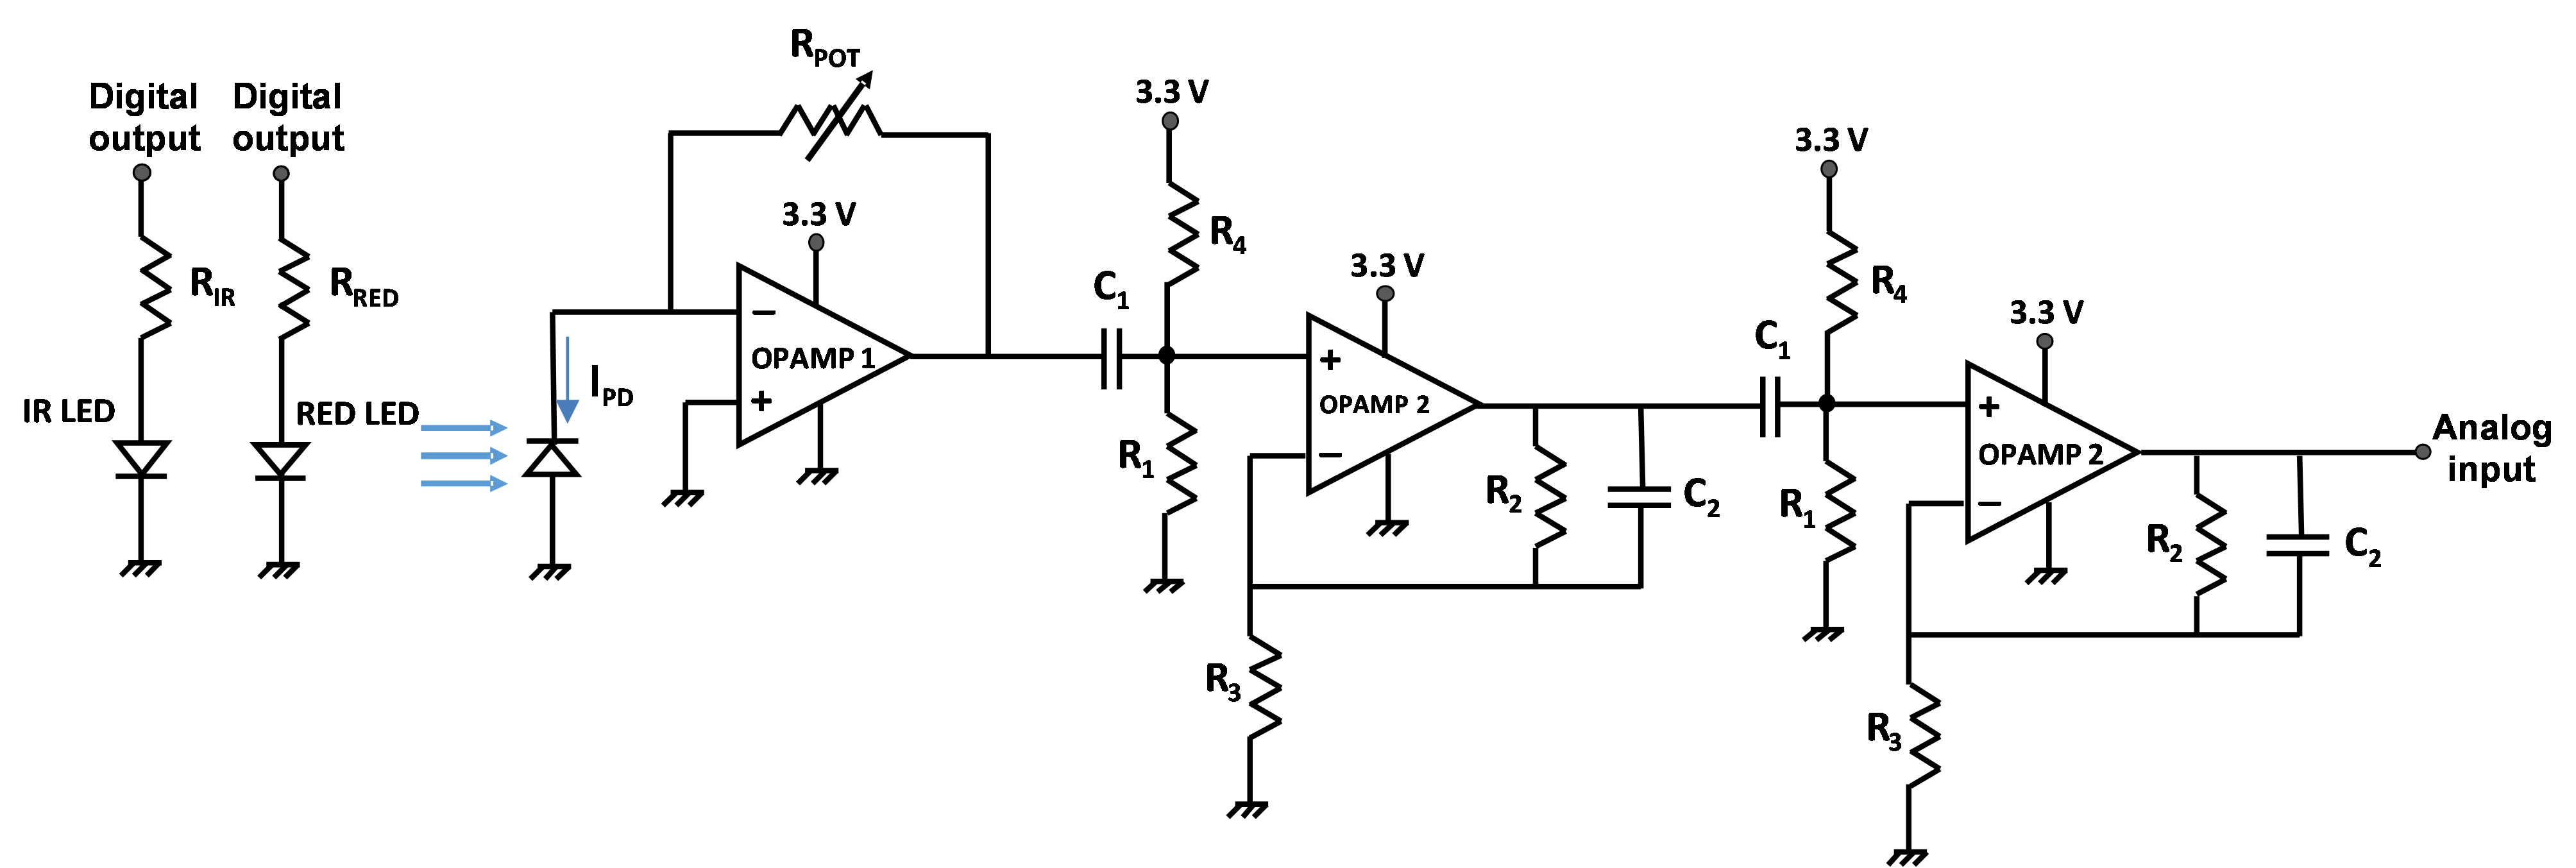
\includegraphics[width=\linewidth]{Circuit1.png}
    \caption{Schema circuito }
    \label{fig:Circuit}
\end{figure}
Il circuito è alimentato mediante porta USB del PC, la quale eroga circa $(\sim 5 V)$. Ed è composto da un primo stadio (OPAMP 1) "in cui si va a regolare l'offset" e un secondo stadio in cui vi è un doppio filtro passa-banda (OPAMP 2) che taglia le frequenze inferiori a 0.8 Hz e superiori a 3 Hz.
\subsection{Dimensionamento resistenze LED}
Dimensioniamo le resistenze $R_{IR},R_{RED}$ in modo da ottenere sui due LED rosso e infrarosso, correnti pari a $I_{RED}=15\text{ mA},I_{IR}=$3 mA rispettivamente. Usando i pin high current della scheda Arduino Due che riescono riescono ad erogare una corrente massima di 15 mA
\begin{equation}
    \frac{V_{CC}-V_{f,IR}}{I_{IR}}=100\text{ }\Omega\quad\frac{V_{CC}-V_{f,RED}}{I_{RED}}=103.33\text{ }\Omega
\end{equation}
Dove i valori della tensione di Forward lì abbiamo reperiti dal datasheet e valgono $V_{f,IR}=3$ V e $V_{f,RED}=1.75$ V.
\subsection{Calcolo funzioni di trasferimento}
Calcoliamo ora la funzione di trasferimento del
\begin{itemize}
    \item Filtro passa-alto costituito da $C_1,R_1,R_4$
    \item Filtro passa-basso costituito da $C_2,R_2,R_3$
    \item Filtro passa-banda complessiva
\end{itemize}
\subsection{Dimensionamento resistenze filtro}
Dimensioniamo le resistenze $R_1, R_2, R_3, R_4$ in modo da ottenere:
\begin{itemize}
    \item Il filtro passa-alto costituito da $C_1, R_1, R_4$ abbia frequenza di taglio pari a 0.8 Hz
    \item La tensione DC a riposo ai morsetti $V_+$ sia pari a 0.15 V
    \item Il filtro passa-basso costituito da $R_2, R_3, C_2$ abbia frequenza di taglio pari a 3 Hz
    \item Il guadagno in DC del filtro passa-basso costituito da $R_2, R_3, C_2$ sia pari a 11   
\end{itemize}
Sceglieremo poi il valore commerciale più vicino per le resistenze $R_1, R_2, R_3, R_4$
\subsection{Tracciamento risposta in frequenza filtro}
Con i valori scelti al punto \ref{}, tracciamo la risposta in frequenza di:
\begin{itemize}
    \item Filtro passa-alto costituito da $C_1,R_1,R_4$
    \item Filtro passa-basso costituito da $C_2,R_2,R_3$
    \item Filtro passa-banda complessiva
\end{itemize}
evidenziando le frequenze di taglio ottenute utilizzando i valori commerciali delle resistenze, necessariamente diverse da 0.8 Hz e 3 Hz